\documentclass[11pt,a4paper]{article}
% Portable pdfLaTeX manuscript; no journal-specific class or shell escape needed.
\usepackage[T1]{fontenc}
\usepackage[utf8]{inputenc}
\usepackage{lmodern,textcomp}
\usepackage[a4paper,margin=22mm,headheight=14pt]{geometry}
\usepackage{amsmath,amssymb}
\usepackage{graphicx,booktabs,array,longtable,tabularx}
\usepackage{xcolor,float,needspace,microtype}
\usepackage[numbers,sort&compress]{natbib}
\usepackage[font=small,labelfont=bf,justification=raggedright,singlelinecheck=false]{caption}
\usepackage{fancyhdr}
\usepackage[hidelinks,unicode]{hyperref}
\urlstyle{same}
\definecolor{missingcolor}{RGB}{155,67,30}
\newcommand{\missing}[1]{{\color{missingcolor}#1}}
\setlength{\parindent}{0pt}
\setlength{\parskip}{5pt plus 1pt minus 1pt}
\setlength{\emergencystretch}{2em}
\setlength{\tabcolsep}{4pt}
\renewcommand{\arraystretch}{1.18}
\linespread{1.08}
\pagestyle{fancy}
\fancyhf{}
\fancyhead[L]{\small MALT versus SS classification}
\fancyhead[R]{\small Research manuscript}
\fancyfoot[C]{\thepage}
\renewcommand{\headrulewidth}{0.3pt}
\renewcommand{\topfraction}{0.95}
\renewcommand{\bottomfraction}{0.95}
\renewcommand{\textfraction}{0.05}
\renewcommand{\floatpagefraction}{0.70}
\setlength{\textfloatsep}{16pt plus 2pt minus 2pt}
\makeatletter
\setlength{\@fptop}{0pt}
\setlength{\@fpsep}{14pt}
\setlength{\@fpbot}{0pt plus 1fil}
\makeatother
\AtBeginEnvironment{table}{\sffamily}

\renewcommand{\thetable}{S\arabic{table}}
\renewcommand{\thefigure}{S\arabic{figure}}
\renewcommand{\theequation}{S\arabic{equation}}
\fancyhead[R]{\small Supplementary information}
\begin{document}
\begin{center}\fbox{\begin{minipage}{.92\textwidth}\small
\textbf{Public repository copy -- filtered, not the complete submission draft.}
Tissue images, individual-slide plots, case-level tables and row-level source data
are withheld. Marked omissions preserve the original numbering and captions.
References to Source Data describe the local research archive; only screened
aggregate tables are distributed here. Reported aggregate estimates are unchanged.
\end{minipage}}\end{center}\medskip
{\Large\bfseries Supplementary information\par}
\medskip
{\large Weakly supervised whole-slide classification of salivary
gland MALT lymphoma versus Sjögren's syndrome\par}
\medskip
Diagnostic counts and estimates correspond to the accompanying main manuscript.
Completion markers identify pending author information, including hospital-held
records awaiting incorporation. Throughout these materials, ``internal evaluation'' or ``holdout'' denotes the 49-slide validation set also used for checkpoint selection, not an independent test. Historical figure assets and numerical results are retained from v7; additional analyses appear in Tables S16--S19. Bold and underlined point estimates denote the best and second-best distinct values, respectively, within each stated comparison group; ties receive the same marking. Rankings are descriptive, not significance tests. All fixed-score intervals omit selection effects and unknown patient clustering.
\begin{table}[H]\centering
\caption{Model configurations}\label{tab:S1}
\small
\begin{tabular}{>{\raggedright\arraybackslash}p{0.367647\dimexpr\textwidth-14\tabcolsep\relax}>{\raggedright\arraybackslash}p{0.073529\dimexpr\textwidth-14\tabcolsep\relax}>{\raggedright\arraybackslash}p{0.088235\dimexpr\textwidth-14\tabcolsep\relax}>{\raggedright\arraybackslash}p{0.117647\dimexpr\textwidth-14\tabcolsep\relax}>{\raggedright\arraybackslash}p{0.088235\dimexpr\textwidth-14\tabcolsep\relax}>{\raggedright\arraybackslash}p{0.117647\dimexpr\textwidth-14\tabcolsep\relax}>{\raggedright\arraybackslash}p{0.147059\dimexpr\textwidth-14\tabcolsep\relax}}
\toprule
\textbf{Model} & \textbf{Seed} & \textbf{Epochs} & \textbf{LR} & \textbf{Batch} & \textbf{Patches} & \textbf{Best epoch} \\
\midrule
Three-model ensemble & 42 & N/A & N/A & N/A & 512 & N/A \\
Hybrid-Evidence MIL & 42 & 30 & 5e-05 & 8 & 512 & 15 \\
ABMIL & 42 & 50 & 5e-05 & 16 & 512 & 37 \\
DTFD-style & 42 & 20 & 5e-05 & 8 & 512 & 11 \\
CLAM-SB-style & 42 & 20 & 5e-05 & 8 & 512 & 16 \\
RRTMIL-style & 42 & 20 & 5e-05 & 4 & 512 & 11 \\
ProtoMIL-style & 42 & 20 & 5e-05 & 8 & 512 & 14 \\
Mean pooling & 42 & 50 & 5e-05 & 16 & 512 & 35 \\
TransMIL-style & 42 & 20 & 5e-05 & 4 & 512 & 14 \\
DSMIL-style & 42 & 20 & 5e-05 & 8 & 512 & 17 \\
Distribution-ProtoMIL & 42 & 20 & 5e-05 & 8 & 512 & 8 \\
CONCH v1.5 + TITAN & 42 & 50 & 5e-05 & 1 & 1024 & 44 \\
\bottomrule
\end{tabular}

\par\medskip\footnotesize All rows refer to the internal MALT/SS task. The ensemble has no separate training epochs.
\end{table}

\begingroup\footnotesize
\renewcommand{\arraystretch}{1.12}
\begin{longtable}{@{}p{.29\textwidth}p{.18\textwidth}p{.45\textwidth}@{}}
\caption{Complete internal interval estimates}\label{tab:S2}\\
\toprule Model & Metric & Estimate (95\% interval) \\ \midrule\endfirsthead
\toprule Model & Metric & Estimate (95\% interval) \\ \midrule\endhead
\midrule\multicolumn{3}{r}{Continued on the next page}\\\endfoot\bottomrule\endlastfoot

Three-model ensemble & AUROC & \textbf{0.9649} (0.9097--1.0000) \\*

 & AUPRC & \textbf{0.9576} (0.8930--1.0000) \\*

 & Accuracy & \underline{87.76\%} (75.76\%--94.27\%) \\*

 & Sensitivity & \underline{91.30\%} (73.20\%--97.58\%) \\*

 & Specificity & 84.62\% (66.47\%--93.85\%) \\*

 & PPV & 84.00\% (65.35\%--93.60\%) \\*

 & NPV & 91.67\% (74.15\%--97.68\%) \\*

 & F1 & 0.8750 (0.7777--0.9583) \\

\addlinespace

Hybrid-Evidence MIL & AUROC & \underline{0.9599} (0.9046--0.9967) \\*

 & AUPRC & \underline{0.9514} (0.8864--0.9965) \\*

 & Accuracy & \underline{87.76\%} (75.76\%--94.27\%) \\*

 & Sensitivity & \textbf{95.65\%} (79.01\%--99.23\%) \\*

 & Specificity & 80.77\% (62.12\%--91.49\%) \\*

 & PPV & 81.48\% (63.30\%--91.82\%) \\*

 & NPV & \underline{95.45\%} (78.20\%--99.19\%) \\*

 & F1 & \underline{0.8800} (0.7925--0.9583) \\

\addlinespace

ABMIL & AUROC & 0.9498 (0.8879--0.9933) \\*

 & AUPRC & 0.9396 (0.8675--0.9928) \\*

 & Accuracy & 85.71\% (73.33\%--92.90\%) \\*

 & Sensitivity & 82.61\% (62.86\%--93.02\%) \\*

 & Specificity & 88.46\% (71.02\%--96.00\%) \\*

 & PPV & 86.36\% (66.67\%--95.25\%) \\*

 & NPV & 85.19\% (67.52\%--94.08\%) \\*

 & F1 & 0.8444 (0.7273--0.9362) \\

\addlinespace

DTFD-style & AUROC & 0.9398 (0.8679--0.9916) \\*

 & AUPRC & 0.9416 (0.8786--0.9922) \\*

 & Accuracy & \underline{87.76\%} (75.76\%--94.27\%) \\*

 & Sensitivity & 86.96\% (67.87\%--95.46\%) \\*

 & Specificity & 88.46\% (71.02\%--96.00\%) \\*

 & PPV & 86.96\% (67.87\%--95.46\%) \\*

 & NPV & 88.46\% (71.02\%--96.00\%) \\*

 & F1 & 0.8696 (0.7619--0.9565) \\

\addlinespace

CLAM-SB-style & AUROC & 0.9365 (0.8612--0.9933) \\*

 & AUPRC & 0.9422 (0.8780--0.9930) \\*

 & Accuracy & \underline{87.76\%} (75.76\%--94.27\%) \\*

 & Sensitivity & \underline{91.30\%} (73.20\%--97.58\%) \\*

 & Specificity & 84.62\% (66.47\%--93.85\%) \\*

 & PPV & 84.00\% (65.35\%--93.60\%) \\*

 & NPV & 91.67\% (74.15\%--97.68\%) \\*

 & F1 & 0.8750 (0.7778--0.9583) \\

\addlinespace

RRTMIL-style & AUROC & 0.9281 (0.8328--0.9967) \\*

 & AUPRC & 0.8400 (0.7022--0.9964) \\*

 & Accuracy & \textbf{89.80\%} (78.24\%--95.56\%) \\*

 & Sensitivity & \textbf{95.65\%} (79.01\%--99.23\%) \\*

 & Specificity & 84.62\% (66.47\%--93.85\%) \\*

 & PPV & 84.62\% (66.47\%--93.85\%) \\*

 & NPV & \textbf{95.65\%} (79.01\%--99.23\%) \\*

 & F1 & \textbf{0.8980} (0.8163--0.9787) \\

\addlinespace

ProtoMIL-style & AUROC & 0.9264 (0.8411--0.9849) \\*

 & AUPRC & 0.9306 (0.8584--0.9862) \\*

 & Accuracy & 85.71\% (73.33\%--92.90\%) \\*

 & Sensitivity & 86.96\% (67.87\%--95.46\%) \\*

 & Specificity & 84.62\% (66.47\%--93.85\%) \\*

 & PPV & 83.33\% (64.15\%--93.32\%) \\*

 & NPV & 88.00\% (70.04\%--95.83\%) \\*

 & F1 & 0.8511 (0.7442--0.9362) \\

\addlinespace

Mean pooling & AUROC & 0.9247 (0.8411--0.9833) \\*

 & AUPRC & 0.9332 (0.8663--0.9851) \\*

 & Accuracy & 85.71\% (73.33\%--92.90\%) \\*

 & Sensitivity & 78.26\% (58.10\%--90.34\%) \\*

 & Specificity & \underline{92.31\%} (75.86\%--97.86\%) \\*

 & PPV & \underline{90.00\%} (69.90\%--97.21\%) \\*

 & NPV & 82.76\% (65.45\%--92.40\%) \\*

 & F1 & 0.8372 (0.7109--0.9362) \\

\addlinespace

TransMIL-style & AUROC & 0.9231 (0.8428--0.9900) \\*

 & AUPRC & 0.9180 (0.8295--0.9891) \\*

 & Accuracy & 81.63\% (68.64\%--90.02\%) \\*

 & Sensitivity & 65.22\% (44.89\%--81.19\%) \\*

 & Specificity & \textbf{96.15\%} (81.11\%--99.32\%) \\*

 & PPV & \textbf{93.75\%} (71.67\%--98.89\%) \\*

 & NPV & 75.76\% (58.98\%--87.17\%) \\*

 & F1 & 0.7692 (0.6061--0.9048) \\

\addlinespace

DSMIL-style & AUROC & 0.9197 (0.8378--0.9816) \\*

 & AUPRC & 0.9260 (0.8579--0.9825) \\*

 & Accuracy & 85.71\% (73.33\%--92.90\%) \\*

 & Sensitivity & 78.26\% (58.10\%--90.34\%) \\*

 & Specificity & \underline{92.31\%} (75.86\%--97.86\%) \\*

 & PPV & \underline{90.00\%} (69.90\%--97.21\%) \\*

 & NPV & 82.76\% (65.45\%--92.40\%) \\*

 & F1 & 0.8372 (0.7027--0.9333) \\

\addlinespace

Distribution-ProtoMIL & AUROC & 0.9130 (0.8227--0.9783) \\*

 & AUPRC & 0.9178 (0.8430--0.9789) \\*

 & Accuracy & 79.59\% (66.36\%--88.52\%) \\*

 & Sensitivity & \underline{91.30\%} (73.20\%--97.58\%) \\*

 & Specificity & 69.23\% (50.01\%--83.50\%) \\*

 & PPV & 72.41\% (54.28\%--85.30\%) \\*

 & NPV & 90.00\% (69.90\%--97.21\%) \\*

 & F1 & 0.8077 (0.7083--0.8980) \\

\addlinespace

CONCH v1.5 + TITAN & AUROC & 0.9013 (0.8026--0.9783) \\*

 & AUPRC & 0.9203 (0.8459--0.9798) \\*

 & Accuracy & 81.63\% (68.64\%--90.02\%) \\*

 & Sensitivity & \underline{91.30\%} (73.20\%--97.58\%) \\*

 & Specificity & 73.08\% (53.92\%--86.30\%) \\*

 & PPV & 75.00\% (56.64\%--87.32\%) \\*

 & NPV & 90.48\% (71.09\%--97.35\%) \\*

 & F1 & 0.8235 (0.7308--0.9167) \\

\addlinespace

\end{longtable}
\endgroup\normalsize

\clearpage

\begin{table}[H]\centering
\caption{Separate ensemble operating point}\label{tab:S3}
\small
\begin{tabular}{>{\raggedright\arraybackslash}p{0.285714\dimexpr\textwidth-4\tabcolsep\relax}>{\raggedright\arraybackslash}p{0.714286\dimexpr\textwidth-4\tabcolsep\relax}}
\toprule
\textbf{Metric} & \textbf{Estimate (95\% interval)} \\
\midrule
AUROC & 0.9649 (0.9097--1.0000) \\
Accuracy & 93.88\% (83.48\%--97.90\%) \\
Sensitivity & 91.30\% (73.20\%--97.58\%) \\
Specificity & 96.15\% (81.11\%--99.32\%) \\
F1 & 0.9333 (0.8511--1.0000) \\
\bottomrule
\end{tabular}

\par\medskip\footnotesize Threshold = 0.70; TN/FP/FN/TP = 25/1/2/21. This is an archived selected operating point.
\end{table}

\begin{table}[H]\centering
\caption{Paired internal model comparisons}\label{tab:S4}
\small
\begin{tabular}{>{\raggedright\arraybackslash}p{0.285714\dimexpr\textwidth-10\tabcolsep\relax}>{\raggedright\arraybackslash}p{0.142857\dimexpr\textwidth-10\tabcolsep\relax}>{\raggedright\arraybackslash}p{0.214286\dimexpr\textwidth-10\tabcolsep\relax}>{\raggedright\arraybackslash}p{0.200000\dimexpr\textwidth-10\tabcolsep\relax}>{\raggedright\arraybackslash}p{0.157143\dimexpr\textwidth-10\tabcolsep\relax}}
\toprule
\textbf{Comparison} & \textbf{AUROC difference} & \textbf{95\% interval} & \textbf{Discordant correct (Hybrid/other)} & \textbf{Exact McNemar P} \\
\midrule
Hybrid minus ABMIL & 0.0100 & -0.0184 to 0.0452 & 4/3 & 1.000 \\
Hybrid minus Three-model ensemble & -0.0050 & -0.0284 to 0.0167 & 1/1 & 1.000 \\
\bottomrule
\end{tabular}

\par\medskip\footnotesize Comparisons use the same 49 WSI and threshold 0.5. No multiplicity adjustment was applied. Intervals use 2,000 paired label-stratified bootstrap samples.
\end{table}

\begin{table}[H]\centering
\caption{External selected subgroups}\label{tab:S5}
\small
\begin{tabular}{>{\raggedright\arraybackslash}p{0.187500\dimexpr\textwidth-12\tabcolsep\relax}>{\raggedright\arraybackslash}p{0.312500\dimexpr\textwidth-12\tabcolsep\relax}>{\raggedright\arraybackslash}p{0.078125\dimexpr\textwidth-12\tabcolsep\relax}>{\raggedright\arraybackslash}p{0.078125\dimexpr\textwidth-12\tabcolsep\relax}>{\raggedright\arraybackslash}p{0.156250\dimexpr\textwidth-12\tabcolsep\relax}>{\raggedright\arraybackslash}p{0.187500\dimexpr\textwidth-12\tabcolsep\relax}}
\toprule
\textbf{Source} & \textbf{Archived stain tag} & \textbf{Label} & \textbf{WSI} & \textbf{Correct at 0.5} & \textbf{Median score} \\
\midrule
MALT\_BJ & H\&E-like & 1 & 33 & 23 & 0.8768 \\
MALT\_BJ & IHC / special stain & 1 & 111 & 111 & 0.8331 \\
MALT\_HE & HE archive & 1 & 8 & 8 & 0.9670 \\
SS\_BJ & SS (slide series) & 0 & 16 & 11 & 0.0543 \\
\bottomrule
\end{tabular}

\par\medskip\footnotesize The initial archive and the selected analysis are separate tables. Filename-derived case counts are not substituted for verified clinical patient counts.
\end{table}

\clearpage

\begin{table}[H]\centering
\caption{Linked performance and interpretation outputs}\label{tab:S6}
\small Individual-case rows are omitted from this public repository copy.
\end{table}

\begin{figure}[H]\centering
\fbox{\begin{minipage}[c][35mm][c]{.88\textwidth}\centering
\textbf{Omitted from this public repository copy}\\[6pt]
This figure contains tissue images or individual-slide observations.\\
The complete figure is retained in the local manuscript archive.
\end{minipage}}
\caption{\textbf{Internal diagnostic-group predictions and threshold behavior}. \textbf{a,} Individual Hybrid scores for the 23 MALT and 26 SS holdout slides. The dashed line marks 0.5. \textbf{b,} Sensitivity and specificity across thresholds for the same fixed predictions. Threshold variation does not represent an additional validation experiment.}\label{fig:S1}\end{figure}

\clearpage
\begin{table}[H]\centering
\caption{Acquisition parameters recovered from archived WSI metadata}\label{tab:S7}
\small
\begin{tabularx}{\textwidth}{@{}>{\raggedright\arraybackslash}Xrrr>{\raggedright\arraybackslash}p{.23\textwidth}@{}}
\toprule
Series & WSIs & Lens & MPP (x/y) & Recorded scanner \\
\midrule
Internal MALT/SS & 193 & $40\times$ & 0.225708 & Hamamatsu C9600-12 \\
External MALT: source B & 144 & $40\times$ & 0.225708 & Hamamatsu C9600-12 \\
External MALT: HE directory & 8 & $40\times$ & 0.225708 & Hamamatsu C9600-12 \\
External SS & 16 & $40\times$ & 0.225708 & Hamamatsu C9600-12 \\
\bottomrule
\end{tabularx}
\par\medskip\footnotesize MPP is in $\mu\mathrm{m}$ per level-0 pixel; the value is equal in both axes. TIFF headers recorded 44,305 pixels per centimetre. Internal files recorded NDP.scan 2.5.85 (133) or 3.3.0 (60); all 168 external files recorded 2.5.85. Coordinate attributes recorded target magnification $20\times$, patch size 512 pixels, level-0 footprint 1,024 pixels and zero overlap for all analyzed files. These metadata describe the archived images; clinical source and stain identities remain subject to provider confirmation.
\end{table}

\begin{table}[H]\centering
\caption{Supporting data and implementation files accompanying the draft}\label{tab:S8}
\small
\begin{tabularx}{\textwidth}{@{}>{\raggedright\arraybackslash}p{.21\textwidth}>{\raggedright\arraybackslash}X>{\raggedright\arraybackslash}p{.25\textwidth}@{}}
\toprule
Material & Contents & Access status \\
\midrule
Source Data draft archive & Publication-coded archived predictions; new same-bag external comparisons, 20-bag sampling outputs and internal-variable diagnostics; all nine controlled training runs, selected epochs and per-slide predictions; provisional reader aggregates; ROI contour and Brier analyses; recovered acquisition metadata. & Accompanies the local author-review draft; public release pending. \\
\addlinespace
Source Code draft archive & Archived custom MIL sources and configurations; new fixed-checkpoint inference and controlled-training runners, prespecified protocols, sampling schedules, dependency/runtime records, metric scripts and publication figure generators. & Accompanies the draft; public repository and licensing pending. \\
\addlinespace
Technical provenance record & Source/configuration/checkpoint and feature-file hashes; archived checkout identity; exact sampled-row indices; current execution metadata distinguished from the unrecovered historical training environment; acquisition and ROI provenance. & Included in the manuscript source package. \\
\addlinespace
Raw WSIs and clinical linkage & Original images, patient/case linkage, clinical characteristics and reference-diagnosis records. & Access arrangements require confirmation by the data-providing institutions. \\
\addlinespace
Individual reader decisions & Per-slide diagnoses, original scores and protocol records. & Held by the hospital data provider; pending incorporation into this draft. \\
\bottomrule
\end{tabularx}
\par\medskip\footnotesize Publication codes identify slides, not patients. The original-identifier mapping and blank clinical/reader confirmation forms are retained locally and excluded from the portable source package. No raw images or model weights are redistributed in these supporting archives.
\end{table}

\clearpage
\begin{table}[H]\centering
\caption{Input activation and gating in the configuration comparison}\label{tab:S9}
\small
\begin{tabularx}{\textwidth}{@{}>{\raggedright\arraybackslash}Xlllr@{}}
\toprule
Configuration & Active vectors & Statistics & Gate & AUROC \\
\midrule
Attention vector & A & Zeroed & Learned & 0.9281 \\
Attention + distribution & A, M, S & Zeroed & Learned & 0.9264 \\
+ high-margin vector + statistics & A, M, S, P & All eight & Learned & \underline{0.9482} \\
Full, equal gate & A, M, S, P, N & All eight & Equal & \textbf{0.9632} \\
Full, learned gate & A, M, S, P, N & All eight & Learned & \underline{0.9482} \\
\bottomrule
\end{tabularx}
\par\medskip\footnotesize Bold/underline denote the highest/second-highest displayed AUROC. A: attention; M: mean; S: standard deviation; P: high-margin vector; N: low-margin instance plus regional vector. Learned gates normalize over five positions, including masked vectors. All configurations retain the Hybrid fusion network. The transition to P also enables the eight statistics. These runs used batch size 16, up to 30 epochs and seed 42; training patch sampling was not fully seed-controlled. Each value is a single run, not a replicate mean. The principal Hybrid run used batch size eight.
\end{table}

\begin{figure}[H]\centering
\fbox{\begin{minipage}[c][35mm][c]{.88\textwidth}\centering
\textbf{Omitted from this public repository copy}\\[6pt]
This figure contains tissue images or individual-slide observations.\\
The complete figure is retained in the local manuscript archive.
\end{minipage}}
\caption{\textbf{Illustrative histological context}. \textbf{a,b,} Supplied MALT and SS photomicrographs, respectively, retained as separate background examples. Source tissue pixels and existing markings were preserved. These are not the model-selected cases in Figure 5. \missing{[MISSING P01: specimen linkage and original calibration; no new physical scale has been inferred.]}}\label{fig:S2}
\end{figure}

\clearpage
\begin{figure}[H]\centering
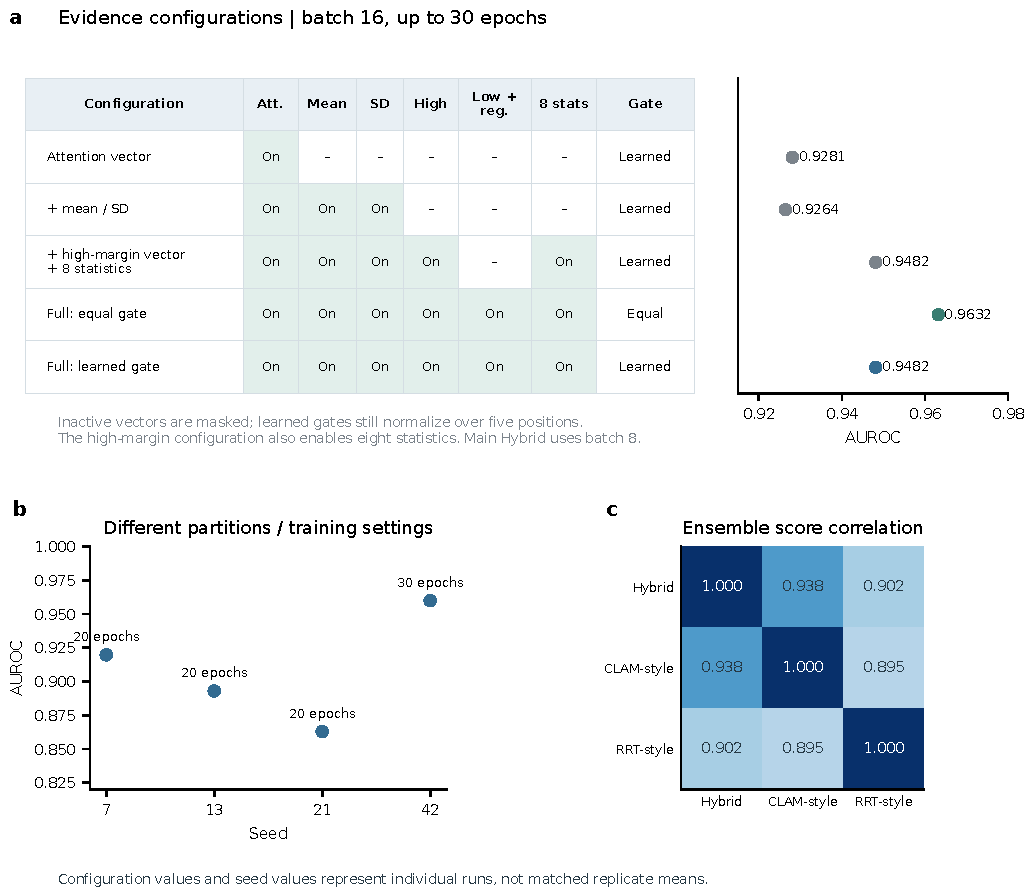
\includegraphics[width=\textwidth,height=.70\textheight,keepaspectratio]{figures/Supplementary_Figure_S3_historical_configurations.pdf}
\caption{\textbf{Historical compound configurations and run records}. \textbf{a,} Input activation matrix and individual configuration AUROCs. Enabling the high-margin vector also enables eight statistics; low-margin and regional vectors remain combined. Learned gates normalize over five positions even when input vectors are masked. These runs used batch size 16 and up to 30 epochs; patch-sampling randomness was not fully seed-controlled. \textbf{b,} Individual runs with different partitions and training settings, retained as historical records rather than matched stability replicates. \textbf{c,} Pearson correlations of ensemble-member scores on the same 49 slides. Every AUROC point represents one run; no replicate error bars are implied. Source data: configuration\_activation\_matrix.csv, ablation\_metrics.csv, seed\_runs.csv and ensemble\_member\_correlations.csv.}\label{fig:S3}
\end{figure}

\clearpage
\begin{table}[H]\centering
\caption{Sampling variability with the fixed Hybrid checkpoint}\label{tab:S10}
\small
\begin{tabular}{p{.47\textwidth}rr}
\toprule
Summary & Internal & External \\
\midrule
WSIs & 49 & 168 \\
Additional bags per WSI & 20 & 20 \\
Median within-slide score SD & 0.0120 & 0.0150 \\
Within-slide score SD, interquartile range & 0.0019--0.0475 & 0.0065--0.0318 \\
Maximum within-slide score SD & 0.1297 & 0.1241 \\
Median within-slide score range & 0.0474 & 0.0581 \\
WSIs crossing 0.5 across the 20 bags & 7/49 & 18/168 \\
SS WSIs crossing 0.5 & 4/26 & 3/16 \\
MALT WSIs crossing 0.5 & 3/23 & 15/152 \\
Per-draw AUROC, mean (SD) & 0.9599 (0.0056) & 0.8749 (0.0097) \\
Per-draw AUROC, range & 0.9498--0.9682 & 0.8549--0.8943 \\
20-bag mean-score AUROC (secondary) & 0.9632 & 0.8775 \\
20-bag mean-score sensitivity (secondary) & 95.65\% & 92.76\% \\
20-bag mean-score specificity (secondary) & 80.77\% & 75.00\% \\
\bottomrule
\end{tabular}
\par\medskip\raggedright\footnotesize Each technical repeat uses 512 sampled feature rows and the same frozen checkpoint. Standard deviations use the sample definition. Crossing means that at least one score is below 0.5 and at least one is at or above 0.5 among the 20 additional bags. AUROC spread across draws is not a confidence interval. Mean-score results are secondary summaries across all 20 bags and do not replace the archived single-bag results. Source data: sampling\_summary.csv, sampling\_per\_slide.csv and sampling\_per\_draw\_metrics.csv.
\end{table}
\clearpage
\begin{table}[H]\centering
\caption{External model comparisons on shared reference bags}\label{tab:S11}
\small
\begin{tabular}{p{.18\textwidth}p{.23\textwidth}p{.23\textwidth}p{.23\textwidth}}
\toprule
Model & AUROC (95\% interval) & Sensitivity (95\% interval) & Specificity (95\% interval) \\
\midrule
Hybrid & \textbf{0.8721} (0.7294--0.9737) & \textbf{93.42\%} (88.31--96.39) & \underline{68.75\%} (44.40--85.84) \\
ABMIL & \underline{0.7903} (0.6275--0.9268) & 42.76\% (35.17--50.71) & \textbf{81.25\%} (56.99--93.41) \\
CLAM-SB-style & 0.6591 (0.4568--0.8491) & 58.55\% (50.60--66.08) & 62.50\% (38.64--81.52) \\
RRTMIL-style & 0.7743 (0.6114--0.9100) & \underline{89.47\%} (83.59--93.42) & 50.00\% (28.00--72.00) \\
\bottomrule
\end{tabular}
\medskip
\begin{tabular}{p{.32\textwidth}rp{.27\textwidth}}
\toprule
Paired difference & AUROC difference & 95\% interval \\
\midrule
Hybrid minus ABMIL & 0.0818 & -0.0136 to 0.2011 \\
Hybrid minus CLAM-SB-style & 0.2130 & 0.0843 to 0.3528 \\
Hybrid minus RRTMIL-style & 0.0979 & 0.0415 to 0.1649 \\
\bottomrule
\end{tabular}
\par\medskip\raggedright\footnotesize Bold/underline mark the highest/second-highest point estimate in each metric column. All four original checkpoints were evaluated on identical per-slide reference bags from 168 WSIs (152 MALT and 16 SS). Sensitivity and specificity use threshold 0.5 and Wilson intervals. AUROC and paired-difference intervals in this new analysis use 10,000 label-stratified WSI bootstrap draws; the archived Hybrid intervals in main Table 3 use 2,000 draws. Differences are unadjusted descriptive comparisons of complete model implementations, not isolated aggregation mechanisms or confirmatory family-wise inference. Source data: reference\_model\_metrics.csv and external\_paired\_comparisons.csv.
\end{table}
\clearpage
\begin{table}[H]\centering
\caption{Archived segmentation-contour coverage of the eight displayed regions}\label{tab:S12}
\small Individual-case rows are omitted from this public repository copy.
\end{table}
\clearpage
\begin{table}[H]\centering
\caption{Descriptive Brier scores of archived predictions}\label{tab:S13}
\small
\begin{tabular}{llrl}
\toprule
Cohort & Model & WSIs & Brier score (95\% interval) \\
\midrule
Internal & Hybrid & 49 & 0.0895 (0.0429--0.1463) \\
Internal & ABMIL & 49 & 0.1056 (0.0396--0.1827) \\
Internal & CLAM-SB-style & 49 & 0.1002 (0.0561--0.1525) \\
Internal & RRTMIL-style & 49 & \underline{0.0894} (0.0341--0.1569) \\
Internal & Three-model ensemble & 49 & \textbf{0.0829} (0.0412--0.1330) \\
External & Hybrid & 168 & 0.0919 (0.0702--0.1156) \\
\bottomrule
\end{tabular}
\par\medskip\raggedright\footnotesize Bold/underline mark the lowest/second-lowest point estimate within each cohort; a lone estimate is unranked. Brier score is the mean squared difference between the uncalibrated sigmoid score and the binary label (MALT = 1). Intervals use 10,000 label-stratified WSI bootstrap resamples of fixed predictions. Seeds are recorded in the source table. No calibration function was fitted to either evaluation cohort. Brier score combines several aspects of probabilistic prediction and does not independently isolate calibration or establish clinical utility. Source data: brier\_descriptive.csv.
\end{table}
\clearpage
\begin{table}[H]\centering
\caption{Dimensions and parameter counts of the evaluated complete models}\label{tab:S14}
\small
\begin{tabular}{lrrrrr}
\toprule
Model & Head input & Attention width & Parameters & Epoch budget & Batch \\
\midrule
Hybrid & 256 & 256 & 1,521,672 & 30 & 8 \\
ABMIL & 1536 & 512 & 6,690,306 & 50 & 16 \\
CLAM-SB-style & 256 & 256 & 591,874 & 20 & 8 \\
RRTMIL-style & 256 & 256 & 1,711,874 & 20 & 4 \\
\bottomrule
\end{tabular}
\par\medskip\raggedright\footnotesize All models receive 1,536-dimensional UNI2-h features and use 512 sampled rows. Head input is the dimension passed from the slide encoder to the common classifier construction; its hidden width is 256. ABMIL retains 1,536-dimensional patch features with additional transformations before and after attention pooling, whereas Hybrid projects features to 256 dimensions and fuses five vectors with eight statistics. These differences, along with training budgets, prevent attribution to pooling alone. Parameter counts were obtained by strict loading of the archived checkpoints; they do not measure runtime, memory, or energy. Source data: model\_checkpoint\_inventory.csv and checkpoint\_tensor\_shapes.json.
\end{table}


\clearpage
\begin{table}[H]\centering
\caption{All predefined controlled training runs}\label{tab:S15}
\small
\begin{tabular}{lrrrrrr}
\toprule
Configuration & Seed & Epoch & \shortstack{Internal\\AUROC} & \shortstack{External\\AUROC} & \shortstack{External\\sensitivity} & \shortstack{External\\specificity} \\
\midrule
Matched attention & 17 & 13 & \textbf{0.9314} & \underline{0.8170} & \textbf{80.26\%} & 62.50\% \\
Matched attention & 29 & 18 & \underline{0.9331} & \underline{0.7500} & \textbf{61.18\%} & 62.50\% \\
Matched attention & 43 & 12 & 0.9398 & 0.6139 & \textbf{34.87\%} & 56.25\% \\
\addlinespace
Fixed scaling & 17 & 24 & 0.9231 & \textbf{0.8701} & 53.29\% & \textbf{87.50\%} \\
Fixed scaling & 29 & 18 & \textbf{0.9431} & 0.7442 & 56.58\% & \underline{68.75\%} \\
Fixed scaling & 43 & 25 & \textbf{0.9532} & \underline{0.6192} & 13.16\% & \underline{62.50\%} \\
\addlinespace
Learned gate & 17 & 29 & \underline{0.9298} & 0.7311 & \underline{60.53\%} & \underline{68.75\%} \\
Learned gate & 29 & 20 & \underline{0.9331} & \textbf{0.9350} & \underline{59.21\%} & \textbf{93.75\%} \\
Learned gate & 43 & 29 & \underline{0.9431} & \textbf{0.6238} & \underline{17.76\%} & \textbf{68.75\%} \\
\addlinespace
\bottomrule
\end{tabular}
\par\medskip\raggedright\footnotesize Bold/underline compare configurations within the same seed and metric column. Each run used the same original 144/49 training/evaluation partition, 30 epochs, batch size eight, learning rate $5\times10^{-5}$, weight decay $10^{-4}$, dropout 0.3 and positive-class loss weight $77/67$. Within each seed, configurations shared identical initial values for common tensors, training bags and minibatch order. The original internal and external reference bags were fixed. Epoch denotes the first epoch with the highest internal AUROC; external evaluation was performed after selection. All nine predefined runs are reported. Matched attention shares the 256-dimensional projection, attention block and classifier construction but omits the other vectors, statistics and fusion layer. Fixed scaling multiplies all five vectors by 0.2; learned gating also changes nonlinear capacity. Parameters: matched attention 658,178, fixed scaling 1,190,403, learned gate 1,521,672. Thus these are controlled configuration comparisons, not parameter-matched or isolated single-component tests. Across-seed summaries describe training variation in the same cohort and do not add independent WSIs. No three-seed significance test is used. Source data: run\_metrics.csv, configuration\_summary.csv and paired\_seed\_differences.csv.
\end{table}

\begin{figure}[H]\centering
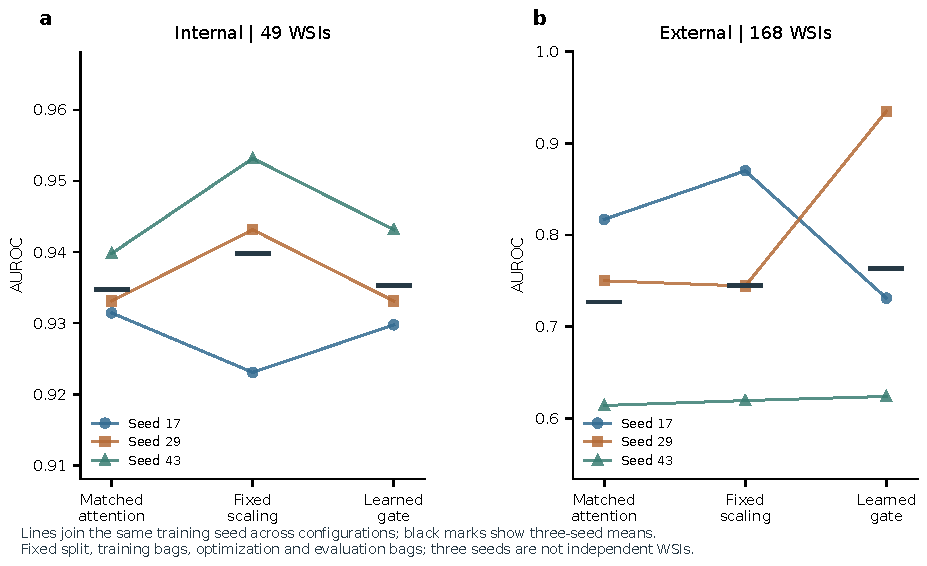
\includegraphics[width=\textwidth,height=.42\textheight,keepaspectratio]{figures/Supplementary_Figure_S4_controlled_training.pdf}
\caption{\textbf{Controlled configuration comparisons across three training seeds}. \textbf{a,b,} Internal and external AUROCs for every selected checkpoint from the nine predefined runs in Supplementary Table S15. Lines join the same seed across configurations and black horizontal marks denote three-seed means. Cohorts and evaluation inputs are unchanged across runs. Three seed values are descriptive training repeats rather than independent clinical observations; no confidence interval or inferential superiority claim is implied. Source data: run\_metrics.csv.}\label{fig:S4}
\end{figure}


% Controlled training results are synthesized in the main Results; S15/Fig. S4 retained.

% Generated by build_development_tables.py; do not hand-edit values.
\clearpage
\begin{table}[H]\centering
\caption{All configurations in the bounded three-seed screen}\label{tab:S16}
\small
\begin{tabularx}{\textwidth}{@{}>{\raggedright\arraybackslash}Xcc@{}}
\toprule
Configuration & Internal AUROC & External AUROC \\
\midrule
Hybrid control & $\underline{0.9353}\pm0.0070$ & $0.7633\pm0.1581$ \\
Matched attention & $0.9348\pm0.0044$ & $0.7270\pm0.1035$ \\
Normalized Hybrid & $0.9337\pm0.0140$ & $0.7166\pm0.2016$ \\
Normalized attention & $\mathbf{0.9365}\pm0.0060$ & $\underline{0.7726}\pm0.1111$ \\
Attention masking & $0.9348\pm0.0073$ & $0.7356\pm0.0940$ \\
Direct attention & $0.9041\pm0.0463$ & $0.6051\pm0.2023$ \\
Subspace attention & $0.8701\pm0.0174$ & $\mathbf{0.7876}\pm0.0617$ \\
Subspace + large batch & $0.8790\pm0.0070$ & $0.7707\pm0.0504$ \\
Hybrid, two bags & $0.9337\pm0.0245$ & $0.6886\pm0.2175$ \\
Hybrid + consistency & $0.9337\pm0.0235$ & $0.7307\pm0.1694$ \\
\bottomrule
\end{tabularx}
\par\medskip\footnotesize Bold/underline mark the highest/second-highest displayed mean within each column. Each cell is mean $\pm$ sample SD across seeds 17, 29 and 43 (30 runs), using the same 49 internal validation and 168 external WSIs. The internal set selected epochs. The control configurations repeat the earlier matched-attention and learned-gate runs and must not be counted as independent clinical replications. Normalized attention was selected among the eight non-control candidates using internal mean AUROC before new external inference. Its internal gain over Hybrid was 0.0011, below the prespecified 0.01 engineering target. The previously examined external collection remains a development evaluation. All configurations, selected epochs, parameter counts, confusion counts and individual seed results are retained in the accompanying CSV files; no external-best selection is implied. Source: screen\_summary.csv and run\_metrics\_verified.csv.
\end{table}

\clearpage
\begin{table}[H]\centering
\caption{Additional seeds, all-five-seed summaries and deterministic linear controls}\label{tab:S17}
\small
\textbf{a, Neural models: seed groups reported separately}\par\smallskip
\begin{tabularx}{\textwidth}{@{}>{\raggedright\arraybackslash}Xlcccc@{}}
\toprule
Model & Seeds & Internal AUROC & External AUROC & Ext. sens. & Ext. spec. \\
\midrule
Hybrid control & 17,29,43 & $\underline{0.9353}\pm0.0070$ & $\underline{0.7633}\pm0.1581$ & \underline{45.83} & \textbf{77.08} \\
Normalized attention & 17,29,43 & $\mathbf{0.9365}\pm0.0060$ & $\mathbf{0.7726}\pm0.1111$ & \textbf{59.65} & \underline{72.92} \\
Hybrid control & 59,71 & $\mathbf{0.9339}\pm0.0248$ & $\mathbf{0.8690}\pm0.0643$ & \textbf{54.28} & \underline{90.62} \\
Normalized attention & 59,71 & $\underline{0.9306}\pm0.0130$ & $\underline{0.8563}\pm0.0218$ & \underline{49.67} & \textbf{93.75} \\
Hybrid control & All five & $\mathbf{0.9348}\pm0.0134$ & $\underline{0.8056}\pm0.1299$ & \underline{49.21} & \textbf{82.50} \\
Normalized attention & All five & $\underline{0.9341}\pm0.0084$ & $\mathbf{0.8061}\pm0.0916$ & \textbf{55.66} & \underline{81.25} \\
\bottomrule
\end{tabularx}
\par\medskip
\textbf{b, Deterministic logistic controls}\par\smallskip
\begin{tabularx}{\textwidth}{@{}>{\raggedright\arraybackslash}Xlcccc@{}}
\toprule
Representation & Inference & Internal AUROC & External AUROC & Ext. sens. & Ext. spec. \\
\midrule
Raw mean + logistic & 512 rows & \textbf{0.9314} & \underline{0.8335} & \underline{45.39} & \textbf{93.75} \\
Raw mean + logistic & All rows & \textbf{0.9264} & \underline{0.8396} & \textbf{45.39} & \textbf{93.75} \\
Normalized mean + logistic & 512 rows & \underline{0.9247} & \textbf{0.8462} & \textbf{46.05} & \textbf{93.75} \\
Normalized mean + logistic & All rows & \underline{0.9247} & \textbf{0.8475} & \underline{44.74} & \textbf{93.75} \\
\bottomrule
\end{tabularx}
\par\medskip\footnotesize Bold/underline mark the highest/second-highest point estimate within each column and matched seed group (panel a) or inference mode (panel b). Neural AUROC cells show means $\pm$ sample SD, not confidence intervals. Sensitivity and specificity are percentages at threshold 0.5; panel a averages each rate across seeds. All-five summaries contain the initial three seeds and the additional two, not five new runs. Selection used only the initial internal results; additional seeds test stability on the same cohort. Each logistic model was fitted once using all-feature means from the 144 training slides and train-only standardization; inference on 512-row reference bags and all available rows is distinguished. No evaluation data were used to fit the scaler or linear coefficients. These are distinct from historical neural mean pooling. Source: confirmation\_summary.csv and linear\_controls.csv. Individual seed outcomes are in selected\_control\_all\_five\_per\_seed.csv.
\end{table}

\clearpage
\begin{table}[H]\centering
\caption{Post hoc archive-tag sensitivity analysis and descriptive error references}\label{tab:S18}
\small
\begin{tabularx}{\textwidth}{@{}>{\raggedright\arraybackslash}Xcc@{}}
\toprule
Metric & Full external set & After tag exclusion \\
\midrule
WSIs & 168 & 57 \\
MALT & 152 & 41 \\
SS & 16 & 16 \\
True positives & 142 & 31 \\
False negatives & 10 & 10 \\
True negatives & 11 & 11 \\
False positives & 5 & 5 \\
AUROC & 0.8721 & 0.8689 \\
Average precision & 0.9733 & 0.9326 \\
Sensitivity (\%) & 93.42 & 75.61 \\
Specificity (\%) & 68.75 & 68.75 \\
Balanced accuracy (\%) & 81.09 & 72.18 \\
Accuracy (\%) & 91.07 & 73.68 \\
NPV (\%) & 52.38 & 52.38 \\
Brier score & 0.0919 & 0.1513 \\
\bottomrule
\end{tabularx}
\par\medskip\footnotesize The excluded 111 slides all had MALT labels and IHC/special-stain archive tags. The remaining 57 slides comprise 33 H\&E-like MALT, eight HE-directory MALT and 16 SS slides with unconfirmed stain. This post hoc calculation retains the historical Hybrid scores and threshold 0.5; it is not confirmed H\&E-only validation and does not isolate a stain effect. All ten external MALT false negatives remain in the subset. No new training or threshold selection was performed.
\par\smallskip For the full 168-slide set, the Brier score of a constant equal to its observed MALT fraction ($152/168$) is 0.0862. This reference uses evaluation labels and is descriptive, not a deployable comparator. A constant equal to the training MALT fraction ($67/144$) has Brier score 0.2793 on the same set. These references contextualize the historical Hybrid score of 0.0919 without establishing calibration. Source: external\_final\_predictions.csv and review\_numeric\_audit.json.
\end{table}

\clearpage
\begingroup\small\sffamily
\begin{longtable}{@{}p{.26\textwidth}p{.24\textwidth}lrrr@{}}
\caption{Prespecified probability aggregation in the bounded development study}\label{tab:S19}\\
\toprule
Model & Aggregation & Set & AUROC & Sens. & Spec. \\
\midrule
\endfirsthead
\multicolumn{6}{l}{\textbf{Supplementary Table S19 (continued)}}\\
\toprule
Model & Aggregation & Set & AUROC & Sens. & Spec. \\
\midrule
\endhead
\midrule\multicolumn{6}{r}{Continued on next page}\\
\endfoot
\bottomrule
\endlastfoot
Hybrid control & 3 seeds, reference & Int. & \underline{0.9482} & \textbf{91.30} & \underline{88.46} \\
Hybrid control & 3 seeds, reference & Ext. & 0.7730 & 40.13 & \textbf{81.25} \\
Matched attention & 3 seeds, reference & Int. & 0.9381 & \textbf{91.30} & 76.92 \\
Matched attention & 3 seeds, reference & Ext. & 0.7171 & 61.18 & 62.50 \\
Normalized Hybrid & 3 seeds, reference & Int. & \textbf{0.9532} & \textbf{91.30} & 76.92 \\
Normalized Hybrid & 3 seeds, reference & Ext. & 0.6982 & 51.32 & 56.25 \\
Normalized attention & 3 seeds, reference & Int. & 0.9431 & 82.61 & \underline{88.46} \\
Normalized attention & 3 seeds, reference & Ext. & 0.7817 & 55.26 & \underline{68.75} \\
Attention masking & 3 seeds, reference & Int. & 0.9415 & \textbf{91.30} & 80.77 \\
Attention masking & 3 seeds, reference & Ext. & 0.7303 & 60.53 & 62.50 \\
Direct attention & 3 seeds, reference & Int. & 0.9365 & \underline{86.96} & \underline{88.46} \\
Direct attention & 3 seeds, reference & Ext. & 0.5095 & 42.11 & 50.00 \\
Subspace attention & 3 seeds, reference & Int. & 0.8612 & 82.61 & 65.38 \\
Subspace attention & 3 seeds, reference & Ext. & \textbf{0.7973} & \textbf{69.08} & \underline{68.75} \\
Subspace + large batch & 3 seeds, reference & Int. & 0.8813 & 78.26 & 76.92 \\
Subspace + large batch & 3 seeds, reference & Ext. & \underline{0.7932} & \underline{62.50} & \underline{68.75} \\
Hybrid, two bags & 3 seeds, reference & Int. & 0.9415 & \textbf{91.30} & 80.77 \\
Hybrid, two bags & 3 seeds, reference & Ext. & 0.6674 & 60.53 & 62.50 \\
Hybrid + consistency & 3 seeds, reference & Int. & \underline{0.9482} & \underline{86.96} & \textbf{92.31} \\
Hybrid + consistency & 3 seeds, reference & Ext. & 0.6970 & 34.21 & \underline{68.75} \\
Hybrid control & 5 seeds, reference & Int. & \textbf{0.9515} & \textbf{91.30} & \textbf{92.31} \\
Hybrid control & 5 seeds, reference & Ext. & \textbf{0.8470} & \underline{47.37} & \textbf{93.75} \\
Normalized attention & 5 seeds, reference & Int. & \underline{0.9365} & \underline{82.61} & \textbf{92.31} \\
Normalized attention & 5 seeds, reference & Ext. & \underline{0.8199} & \textbf{53.29} & \underline{81.25} \\
Hybrid control & 3 seeds, 5 bags & Int. & \textbf{0.9515} & \textbf{91.30} & \textbf{88.46} \\
Hybrid control & 3 seeds, 5 bags & Ext. & \underline{0.7763} & \underline{41.45} & \textbf{87.50} \\
Normalized attention & 3 seeds, 5 bags & Int. & \underline{0.9465} & \underline{86.96} & \underline{84.62} \\
Normalized attention & 3 seeds, 5 bags & Ext. & \textbf{0.7965} & \textbf{55.26} & \underline{75.00} \\
Hybrid control & 5 seeds, 5 bags & Int. & \textbf{0.9548} & \textbf{91.30} & \textbf{92.31} \\
Hybrid control & 5 seeds, 5 bags & Ext. & \textbf{0.8479} & \underline{48.03} & \textbf{93.75} \\
Normalized attention & 5 seeds, 5 bags & Int. & \underline{0.9381} & \textbf{91.30} & \underline{88.46} \\
Normalized attention & 5 seeds, 5 bags & Ext. & \underline{0.8314} & \textbf{53.95} & \underline{87.50} \\
\end{longtable}
\footnotesize Bold/underline compare models within the same aggregation rule, cohort and metric. Each row is the metric of averaged probabilities, not an average of seed-level metrics. Three seeds are 17/29/43; five seeds additionally include 59/71. Reference denotes the fixed historical 512-row bag. Five-bag aggregation averages five additional bag probabilities within each seed before seed averaging. Subspace configurations additionally average logits across 21 feature windows within each bag. Int.: 49-slide internal validation set; Ext.: historical 168-slide external set. Sensitivity and specificity are percentages at 0.5. These secondary rules were specified before new external inference, but the cohort was previously examined. No row replaced the historical primary checkpoint. Source: ensemble\_metrics.csv; per-seed five-bag results, individual scores and conditional intervals are included in Source Data.
\endgroup

\clearpage
\section*{Supplementary results: additional model development}

Nine controlled runs compared matched attention, full fixed scaling and full learned gating using seeds 17, 29 and 43 (Supplementary Table S15; Fig. S4). Internal AUROC means $\pm$ sample standard deviations were $0.9348\pm0.0044$, $0.9398\pm0.0153$ and $0.9353\pm0.0070$, respectively. Corresponding external values were $0.7270\pm0.1035$, $0.7445\pm0.1254$ and $0.7633\pm0.1581$. The gate comparison showed no consistent advantage across seeds, and the configurations differed in parameter count. Historical compound ablations remain separately documented in Supplementary Table S9 and Fig. S3.

A subsequent bounded study completed 34 neural training runs: ten configurations at three initial seeds, followed by two additional seeds for the internally selected candidate and the Hybrid control (Supplementary Tables S16 and S17). The screen included normalized embeddings, attention masking, direct/subspace attention and two-bag training. It reproduced the original matched-attention and Hybrid controls; these repeated controls are not additional independent clinical evidence. Normalized attention ranked first among eight candidates on mean internal AUROC. Its improvement over Hybrid was 0.0011, below the protocol's 0.01 target. Candidate selection was locked before new external predictions, although this external collection had already been examined in earlier development.

Across all five seeds (17, 29, 43, 59 and 71), internal AUROC was $0.9348\pm0.0134$ for Hybrid and $0.9341\pm0.0084$ for normalized attention. External AUROC was $0.8056\pm0.1299$ and $0.8061\pm0.0916$, respectively. Mean external sensitivities at threshold 0.5 were 49.21\% and 55.66\%, with specificities of 82.50\% and 81.25\%. Thus, the historical primary checkpoint's operating point did not characterize the retrained models. Additional-seed results are reported separately in Supplementary Table S17; no favorable seed replaced the primary checkpoint.

Train-only logistic regression on mean UNI2-h features achieved internal/external AUROCs of 0.9314/0.8335 on the reference bags. Averaging normalized patch features before logistic regression gave 0.9247/0.8462. External sensitivities were 45.39\% and 46.05\%, respectively, at specificity 93.75\% for both. These simple controls retained discrimination but showed a different threshold tradeoff. Complete run metrics, full-feature inference and prespecified aggregation analyses accompany Supplementary Tables S16, S17 and S19. The experiments did not establish a stable advantage of the more complex architecture.


\clearpage
\section*{Supplementary Methods}
\setcounter{subsection}{0}
\renewcommand{\thesubsection}{SM\arabic{subsection}}
Detailed implementation and provenance accompany the main Methods. Internal evaluation always denotes the validation set used for checkpoint selection; later external analyses reuse a historically examined collection.

\subsection{WSI preprocessing and feature extraction}

WSI preprocessing used TRIDENT, with GrandQC tissue segmentation \citep{ref12}. Acquisition parameters were recovered from the archived WSI headers and coordinate-file attributes. All 193 internal and 168 analyzed external WSIs recorded Hamamatsu C9600-12 as the scanner model, a \(40\times\) source-lens setting and a level-0 resolution of approximately \(0.225708\,\mu\mathrm{m}\) per pixel in both axes. The original TIFF resolution tags were 44,305 pixels per centimetre. Internal files recorded NDP.scan versions 2.5.85 (133 WSIs) or 3.3.0 (60 WSIs), and all analyzed external files recorded version 2.5.85. These are file-recorded acquisition parameters; clinical provenance and stain identities are addressed separately. Supplementary Table S7 summarizes the recovered metadata.

Tissue regions were tiled at target magnification \(20\times\) into non-overlapping 512 \(\times\) 512-pixel patches. The archived HDF5 attributes consistently recorded a corresponding 1,024 \(\times\) 1,024-pixel level-0 footprint and zero overlap. Patch features and coordinates were stored in HDF5 files.

The principal experiments used UNI2-h embeddings with 1,536 dimensions per patch. The UNI family provides general-purpose pathological representations \citep{ref8}; the UNI2-h model card identifies the specific encoder family \citep{ref29}. The archived encoder implementation resized the shorter image side to 224 pixels, applied a 224 \(\times\) 224 centre crop, converted images to tensors and normalized RGB channels with means (0.485, 0.456, 0.406) and standard deviations (0.229, 0.224, 0.225). Its configuration specified a ViT-giant encoder with 14-pixel internal token patches, 24 transformer layers, 24 attention heads, eight register tokens and bfloat16 inference precision. The 14-pixel token size is distinct from the WSI extraction patch size. \missing{[MISSING M01: recover the exact UNI2-h weight-file checksum and downloaded checkpoint revision used for feature extraction.]} The image encoder was not fine-tuned within the downstream MIL experiment because training used precomputed embeddings. Each WSI contributed 512 sampled feature vectors. Sampling was without replacement when sufficient instances were available and with replacement otherwise. Training sampling varied across loading events, while inference sampling used deterministic seeds.

CONCH v1.5 with TITAN was evaluated as a separate comparison \citep{ref13}. It used 768-dimensional patch features and 1,024 sampled instances per WSI. Thus, its encoder, patch budget and aggregation strategy differed from those of the UNI2-h comparisons. The corresponding result is identified separately in main Figure 2 and Table 2.

% Restored from ../methods_hybrid_evidence_mil.tex and checked against
% ../../scripts/ss_experiment_suite.py: GatedAttentionPool,
% HybridEvidenceMILEncoder and SlideClassifier. This file is maintained by hand.
\subsection{Hybrid-Evidence MIL}

\paragraph{Task formulation and feature projection.}
Each WSI was represented by a sampled feature bag
$X=\{\mathbf{x}_i\}_{i=1}^{N}$ and its associated patch coordinates
$(a_i,b_i)$, where $N=512$ and $\mathbf{x}_i\in\mathbb{R}^{1536}$.
The slide label was $y=1$ for MALT and $y=0$ for SS.
No patch-level labels were used. A shared projection placed all features in a
$D=256$ dimensional hidden space:
\begin{equation}\label{eq:projection}
 \mathbf{h}_i = \operatorname{Dr}_{0.3}\!\left[
  \operatorname{GELU}\!\left(\operatorname{LN}
  (\mathbf{W}_{p}\mathbf{x}_i+\mathbf{b}_{p})\right)\right],
 \qquad \mathbf{h}_i\in\mathbb{R}^{D}.
\end{equation}
Here $\operatorname{LN}$ denotes layer normalization and $\operatorname{Dr}_{0.3}$
denotes dropout with probability 0.3 during training; dropout is disabled during
inference. All vectors below are column vectors, and $[\,\cdot\,;\,\cdot\,]$
denotes concatenation along the feature dimension.

\paragraph{Gated attention evidence.}
Gated pooling followed the attention mechanism of Ilse and colleagues
\citep{ref5}, with an additional value transformation implemented in the archived
model. For a sequence $Z=\{\mathbf{z}_j\}_{j=1}^{L}$ of $D$ dimensional vectors,
define the pooling operator $\mathcal{G}_{\theta}$ as
\begin{subequations}\label{eq:gated-pool}
\begin{align}
 \mathbf{t}_j &= \operatorname{Dr}_{0.3}
     \!\left[\operatorname{ReLU}(\mathbf{W}_{v}\mathbf{z}_j+\mathbf{b}_{v})\right],
     \label{eq:pool-value}\\
 \ell_j &= \mathbf{w}_{a}^{\mathsf T}
    \left[\tanh(\mathbf{V}\mathbf{t}_j+\mathbf{b}_{V})
     \odot\operatorname{sigmoid}(\mathbf{U}\mathbf{t}_j+\mathbf{b}_{U})\right]+b_a,
     \label{eq:pool-logit}\\
 \alpha_j &= \frac{\exp(\ell_j)}{\sum_{l=1}^{L}\exp(\ell_l)},
 \qquad \mathcal{G}_{\theta}(Z)=\sum_{j=1}^{L}\alpha_j\mathbf{t}_j.
     \label{eq:pool-sum}
\end{align}
\end{subequations}
The symbol $\odot$ denotes element-wise multiplication. All attention and value
matrices map between $D$ dimensional spaces. The attention evidence vector was
$\mathbf{e}_{\mathrm{att}}=\mathcal{G}_{\theta_A}(\{\mathbf{h}_i\}_{i=1}^{N})$.
Thus, the pooling weights multiply transformed values $\mathbf{t}_i$.
The regional branch used the same operator with independently learned parameters
$\theta_R$.

\paragraph{Distribution evidence.}
The center and heterogeneity of the sampled bag were summarized by two separate
vectors:
\begin{subequations}\label{eq:distribution}
\begin{align}
 \mathbf{e}_{\mu} &= \frac{1}{N}\sum_{i=1}^{N}\mathbf{h}_i,\\
 \mathbf{e}_{\sigma} &=
 \left[\frac{1}{N-1}\sum_{i=1}^{N}
       (\mathbf{h}_i-\mathbf{e}_{\mu})^{\odot 2}\right]^{\odot 1/2}.
\end{align}
\end{subequations}
Powers and square roots in Eq.~\eqref{eq:distribution} are element-wise. The
sample denominator $N-1$ matches the standard deviation used in the code.

\paragraph{Prototype-margin evidence.}
Two latent prototype banks indexed by $c\in\{0,1\}$ each contained
$K=8$ learnable prototypes
$\mathbf{p}_{c,r}\in\mathbb{R}^{D}$. Let a hat denote the implemented
$\ell_2$ normalization, with its numerical safeguard for zero norms.
The maximum cosine similarity within each bank and the bank-1-minus-bank-0 margin
were
\begin{subequations}\label{eq:prototype}
\begin{align}
 s_{i,c} &= \max_{1\leq r\leq K}
       \widehat{\mathbf{h}}_i^{\mathsf T}\widehat{\mathbf{p}}_{c,r},
       \qquad m_i=s_{i,1}-s_{i,0},\label{eq:margin}\\
 k &= \min(32,N),\qquad
 I_{+}=\operatorname{TopKIdx}(\{m_i\},k),\qquad
 I_{-}=\operatorname{TopKIdx}(\{-m_i\},k),\\
 \mathbf{e}_{+} &= \frac{1}{k}\sum_{i\in I_{+}}\mathbf{h}_i,
 \qquad \mathbf{e}_{-}=\frac{1}{k}\sum_{i\in I_{-}}\mathbf{h}_i.
\end{align}
\end{subequations}
$\operatorname{TopKIdx}$ returns indices of the $k$ largest entries. The high-
and low-margin vectors therefore average the instances with the largest and
smallest margins, respectively; the selected values need not all have the same
sign. Prototypes were optimized through differentiable similarity and margin
statistics in the slide-level classification objective. The hard top-$k$ index
selections were discrete; no additional prototype-specific loss or regional
labels were used. The bank indices do not identify validated MALT or SS
morphology, and a larger margin is not constrained to increase the final MALT score.

\paragraph{Coordinate-ordered groups and low-margin evidence.}
To form coordinate-ordered groups, let $\pi$ be the permutation obtained by
sorting the implemented coordinate key $10^6b_i+a_i$. The ordered hidden
sequence was partitioned using the code's chunk operation into $Q\leq16$
consecutive non-empty chunks $C_j$ (16 equal chunks for the 512 sampled patches).
Group tokens and the combined low-margin/regional vector were
\begin{subequations}\label{eq:regional}
\begin{align}
 \mathbf{r}_j &= \frac{1}{|C_j|}\sum_{l\in C_j}\mathbf{h}_{\pi(l)},
        \qquad j=1,\ldots,Q,\\
 \mathbf{e}_{\mathrm{reg}} &=
       \mathcal{G}_{\theta_R}(\{\mathbf{r}_j\}_{j=1}^{Q}),
       \qquad \mathbf{e}_{\mathrm{nr}}=\mathbf{e}_{-}+\mathbf{e}_{\mathrm{reg}}.
\end{align}
\end{subequations}
The regional operator includes its own value transformation from
Eq.~\eqref{eq:pool-value}. Coordinates determine group membership, but the
subsequent pooling is invariant to the order of the group tokens. The branch
has no explicit intergroup distances, adjacency or positional encoding.
Equal-sized groups of sampled instances were not anatomical regions and can
span different physical extents.

\paragraph{Similarity and margin statistics.}
Eight scalar statistics supplemented the evidence vectors. Define
$T_c=\operatorname{TopKIdx}(\{s_{i,c}\},k)$,
$\bar{s}_{c}^{\mathrm{top}}=k^{-1}\sum_{i\in T_c}s_{i,c}$ and
$\bar{m}=N^{-1}\sum_i m_i$. Then
\begin{subequations}\label{eq:statistics}
\begin{align}
 s_m &= \left[\frac{1}{N-1}\sum_{i=1}^{N}(m_i-\bar m)^2\right]^{1/2},\\
 \rho_0 &= \frac{1}{N}\sum_{i=1}^{N}\mathbb{I}(m_i>0),\qquad
 \rho_{\bar m}=\frac{1}{N}\sum_{i=1}^{N}\mathbb{I}(m_i>\bar m),\\
 \mathbf{u} &= \bigl[\bar{s}_{0}^{\mathrm{top}},\bar{s}_{1}^{\mathrm{top}},
       \bar m,s_m,\max_i m_i,\min_i m_i,\rho_0,\rho_{\bar m}\bigr]^{\mathsf T}
       \in\mathbb{R}^{8}.
\end{align}
\end{subequations}
$\mathbb{I}$ is the indicator function. The top-similarity sets $T_c$ are computed
separately for the two banks and need not coincide with the margin-based sets
$I_{+}$ and $I_{-}$.

\paragraph{Learned gating, weighted concatenation and classification.}
The five evidence vectors were ordered as
$(\mathbf{e}_1,\ldots,\mathbf{e}_5)=
(\mathbf{e}_{\mathrm{att}},\mathbf{e}_{\mu},\mathbf{e}_{\sigma},
 \mathbf{e}_{+},\mathbf{e}_{\mathrm{nr}})$.
A two-layer gate received the unweighted vectors and statistics:
\begin{subequations}\label{eq:fusion}
\begin{align}
 \mathbf{q} &= [\mathbf{e}_1;\mathbf{e}_2;\mathbf{e}_3;\mathbf{e}_4;
                   \mathbf{e}_5;\mathbf{u}]\in\mathbb{R}^{5D+8},\\
 \boldsymbol{\gamma} &= \operatorname{softmax}\!\left(
    \mathbf{W}_{g2}\operatorname{Dr}_{0.3}\!\left[
       \operatorname{GELU}(\mathbf{W}_{g1}\mathbf{q}+\mathbf{b}_{g1})\right]
       +\mathbf{b}_{g2}\right)\in\mathbb{R}^{5},\label{eq:gate}\\
 \widetilde{\mathbf{q}} &= [\gamma_1\mathbf{e}_1;\gamma_2\mathbf{e}_2;
       \gamma_3\mathbf{e}_3;\gamma_4\mathbf{e}_4;\gamma_5\mathbf{e}_5;
       \mathbf{u}],\label{eq:weighted-concat}\\
 \mathbf{z} &= \operatorname{Dr}_{0.3}\!\left[
       \operatorname{GELU}\!\left(\operatorname{LN}
       (\mathbf{W}_{f}\widetilde{\mathbf{q}}+\mathbf{b}_{f})\right)\right],\\
 a &= \mathbf{w}_{o}^{\mathsf T}\operatorname{Dr}_{0.3}\!\left[
       \operatorname{ReLU}\!\left(\operatorname{LN}
       (\mathbf{W}_{c}\mathbf{z}+\mathbf{b}_{c})\right)\right]+b_o,
       \qquad p=\operatorname{sigmoid}(a).
\end{align}
\end{subequations}
The gate dimensions were $\mathbf{W}_{g1}\in\mathbb{R}^{D\times(5D+8)}$
and $\mathbf{W}_{g2}\in\mathbb{R}^{5\times D}$;
$\mathbf{W}_{f}\in\mathbb{R}^{D\times(5D+8)}$ and
$\mathbf{W}_{c}\in\mathbb{R}^{D\times D}$.
Each $\gamma_j$ is non-negative and $\sum_j\gamma_j=1$.
Equation~\eqref{eq:weighted-concat} preserves five weighted feature blocks;
the eight statistics enter fusion without multiplication by a branch weight.
The gate supplies sample-dependent feature scaling, rather than a distribution
of causal contributions. Branch norms, the learned fusion transformation and
the ungated statistics also affect the classifier. The output $p$ is an
uncalibrated MALT model score in $[0,1]$.

\paragraph{Training objective.}
For a minibatch $\mathcal{B}$ of slides, the weighted binary cross-entropy was
\begin{equation}\label{eq:loss}
 \mathcal{L}=-\frac{1}{|\mathcal{B}|}\sum_{b\in\mathcal{B}}
 \left[w_{+}y_b\log p_b+(1-y_b)\log(1-p_b)\right],
 \qquad w_{+}=\frac{77}{67}.
\end{equation}
The implementation evaluated this objective directly from logits for numerical
stability. The positive-class weight was the ratio of the 77 SS to 67 MALT
training slides. Class weighting changes the optimum of binary cross-entropy;
the sigmoid output was not assumed to equal an unweighted posterior probability.
No calibration model was fitted to either evaluation set. Optimization and the
archived checkpoint are described in the main Methods.


\subsection{Fixed-checkpoint comparison and repeated input sampling}

The fixed-checkpoint analyses reused the four archived Hybrid, ABMIL, CLAM-SB-style and RRTMIL-style checkpoints without updating their weights or extracting new image features. A recorded protocol specified the original 49 internal and 168 external evaluation slides, a common threshold of 0.5 and the sampling analyses before inspection of the new outputs. Reference bags were reconstructed using the historical row indices and sampling rules. In particular, the original full external-manifest indices were retained when evaluating the final subset. All four internal outputs and the archived external Hybrid outputs reproduced to a maximum absolute score difference of $1.20\times10^{-7}$, with identical classifications at 0.5. The three comparators were then evaluated on exactly the same external feature bags as Hybrid.

Sampling sensitivity was measured with 20 additional 512-instance bags for every evaluation WSI, using the fixed Hybrid checkpoint in evaluation mode. For each slide and repeat 1--20, the NumPy random-number seed was the unsigned 32-bit integer represented by the first four bytes, in little-endian order, of the SHA-256 digest of \texttt{20261104|\allowbreak{}scope|\allowbreak{}study\_slide\_id|\allowbreak{}repeat\_id}. Sampling used replacement only when fewer than 512 feature rows were available. As in the historical implementations, indices were sorted only for internal slides with at least 512 rows. Exact indices, seeds, feature-row counts and sampled unique-row counts were saved.

For each slide we calculated the sample standard deviation, minimum and maximum of the 20 scores. A threshold-crossing slide had at least one score below 0.5 and at least one at or above 0.5 among those draws. Complete-cohort AUROC was calculated separately for each repeat. The distribution across draws measures technical input-sampling variation; it is not a confidence interval, an estimate of training variability or an increase in biological sample size. Averaging the 20 scores per slide was evaluated descriptively as a secondary result, without replacing the archived primary predictions.

On each reference bag, a separate instrumented forward calculation recorded latent-bank margins, prototype winner counts, gate scalings and vector norms. Its logits agreed with the original forward calculation within $10^{-5}$. Spearman correlations related the bag-mean margin to the output score and binary label. No regional annotations or causal interpretations were assigned to these internal quantities.

External complete-model AUROC differences used 10,000 class-stratified paired WSI bootstrap draws with seed 20261104 and fixed reference inputs. Each draw sampled the same slides for all models. Percentile intervals and exact paired McNemar tests were descriptive and unadjusted for multiple comparisons. Supplementary Table S11 uses this new 10,000-draw procedure, while the original primary Hybrid intervals are retained from the historical 2,000-draw analysis.


\subsection{Pathologist comparison and interpretation materials}

The available reader material comprised aggregate confusion counts for two pathologists. Individual decisions and the actual review conditions are held by the hospital data provider and await incorporation. The available aggregate counts are retained as provisional summaries pending reconciliation with those records. \missing{[MISSING R01: hospital-held individual reader decisions and protocol, including experience, randomization, blinding and case presentation; pending incorporation.]} Paired performance analyses remain unfilled pending record import. Reading time, confidence and assisted outcomes will only be reported if supported by the original study records.

The reader-analysis specification uses the same WSI-level diagnostic metric definitions and Wilson proportion intervals as the model analysis. Once matched reader records are available, reader--model error overlap and exact McNemar comparisons can be calculated on the same slides. These reader comparisons have not been performed from the provisional aggregates. Confidence-score ROC analysis requires the original reader scores; binary reader decisions alone will be reported through their corresponding diagnostic operating point.

Interpretation used saved case scores, gate weights, prototype-margin overlays and ranked tissue thumbnails. Four displayed cases represent a true positive, true negative, false positive and false negative at threshold 0.5. The performance and interpretation scripts each sampled 512 patches, using seed 42 plus a row index. Performance sampling indexed the evaluation subset; interpretation sampling indexed the full cohort table. Consequently, the sampled bags could differ. Supplementary Table S6 links both archived scores; the original figure outputs were linked without regenerating them.

The margin overlays retain their original pixels and depict sampled patch locations. High and low values describe relative similarity to two latent prototype banks, without assigning either color a verified disease morphology. Colors used a symmetric range $[-s,s]$, where $s=\max(|Q_{0.02}(m)|,|Q_{0.98}(m)|,10^{-6})$ within each slide. The figure legend displays normalized margin $m/s$, with color saturation beyond $\pm1$. Color intensity is therefore not directly comparable across slides. The six continuous similarity/margin statistics provide differentiable paths for prototype optimization. The two indicator proportions and hard top-$k$ indices are discrete operations.

Photomicrographs and ranked tissue thumbnails were reused without contrast, brightness or local image enhancement. Each thumbnail originated from a 1,024 $\times$ 1,024-pixel level-0 window spanning approximately 231.1 $\times$ 231.1 $\mu\mathrm{m}$. This calibration supports 50-$\mu\mathrm{m}$ bars on the model-selected thumbnails, which were stored at 220 $\times$ 220 pixels. For all eight displayed windows, the original 1,024-pixel RGB region resized to 220 pixels by Lanczos resampling matched the archived thumbnail pixel for pixel. Locator boxes use the archived overlay geometry. For Case 10, the archived coordinate metadata recorded a slide height of 62,208 pixels, whereas the current OpenSlide reader reported 70,400 pixels; both widths were 102,400 pixels. The original overlay and its coordinate geometry were retained rather than treating the current reader extent as a newly verified match. This calibration does not apply to the separate illustrative photomicrographs. \missing{[MISSING P01/P03: specimen linkage and original calibration for the illustrative photomicrographs, and pathology-confirmed regional descriptions.]}

Automated segmentation-contour coverage was audited for the same eight windows (Supplementary Table S12). Coverage was the area of the intersection between the union of archived segmentation polygons and the level-0 1,024 $\times$ 1,024-pixel window, divided by the window area. The original segmentation used $1\times$ magnification and treated polygon holes as tissue. This geometric overlap is an automated-mask measure, not a pathologist-confirmed tissue fraction. No ROI was removed or replaced on the basis of the audit; regional pathological interpretation remains pending hospital record incorporation.


\subsection{Component analyses}

Five configurations compared combinations of evidence vectors within the Hybrid architecture (Supplementary Table S9). Each used up to 30 epochs, batch size 16, learning rate $5\times10^{-5}$ and seed 42. When fewer than four vectors were active, all eight similarity/margin statistics were zeroed. Thus, the high-margin configuration simultaneously enabled that vector and the eight statistics. The final vector combined low-margin instances and coordinate-group summaries, without separating their contributions. Inactive vectors were masked, but learned gates retained a softmax over five output positions. The attention-vector configuration therefore retained the Hybrid gate and fusion architecture and was not identical to ABMIL. In the full equal-gate configuration, all five vectors were multiplied by 0.2 before concatenation. A fixed nonzero scaling can be absorbed into the subsequent linear fusion weights in the represented function class, although the parameterization can still affect optimization and regularization.

The seed controlled partitioning and the initialized global random-number streams. However, the component-training dataset created an unseeded NumPy \texttt{default\_rng()} for each training patch sample. It therefore did not fully fix patch-sampling randomness across runs. These results describe the saved configurations, rather than controlled attribution of independent components or exactly reproducible training trajectories.

The archived seed analysis contained seeds 7, 13, 21 and 42. The first three runs allowed 20 epochs and seed 42 allowed 30 epochs. We reported individual AUROCs without treating the four runs as interchangeable repetitions. These historical runs are shown in Supplementary Fig. S3. Ensemble behavior was described by aligned score correlations and by the individual errors corrected, introduced or shared at threshold 0.5.


\subsection{Controlled comparison across training seeds}

A separate protocol specified three configurations and training seeds 17, 29 and 43, for nine runs. Matched attention used the same 1,536-to-256 projection, gated attention block and 256-input classification head as Hybrid, while omitting the other vectors, statistics and fusion layer. Fixed scaling retained all five vectors, the eight statistics and the fusion layer, with each vector multiplied by 0.2 and no trainable gate. Learned gating used the full original Hybrid architecture. Shared tensors started from identical freshly initialized values within each seed. These configurations were not parameter-matched, and the fixed-versus-learned gate comparison also changed nonlinear capacity.

All runs used the existing 144/49 split, 30 epochs, batch size eight, AdamW with learning rate $5\times10^{-5}$ and weight decay $10^{-4}$, dropout 0.3 and positive BCE weight 77/67. The first epoch achieving a strictly higher internal AUROC than all preceding epochs was retained, and final-epoch checkpoints were also archived. External predictions used the selected checkpoint and were computed after selection. There was no early stopping, learning-rate scheduler or calibration fitting.

For each seed and epoch, the configurations received identical sampled training bags and minibatch orders. Bag seeds were the first four little-endian SHA-256 bytes of \texttt{controlled-v6|\allowbreak{}seed|\allowbreak{}epoch|\allowbreak{}study\_slide\_id}; order seeds replaced the slide code with \texttt{order}. PyTorch batch seeds used \texttt{controlled-v6|\allowbreak{}seed|\allowbreak{}epoch|\allowbreak{}batch\_index|\allowbreak{}dropout}. These reset common random streams, although dropout masks after divergent computational branches were not assumed to be elementwise matched. Exact indices and minibatch orders were saved, deterministic algorithms were enabled, and parameter-gradient connectivity was checked in the first minibatch of each run. Internal and external evaluation used the same fixed reference bags as the checkpoint analyses above.

The nine predefined runs were reported individually, with configuration means and sample standard deviations and paired per-seed AUROC differences (Supplementary Table S15). The three seeds describe training variation on the fixed cohort. They were not used as independent clinical observations or to establish inferential significance. The original ABMIL implementation and all historical checkpoint results remained separate.


\subsection{Statistical analysis and figure generation}

The primary display threshold was 0.5. Archived optimized thresholds were reported separately and were not relabeled as prespecified. AUROC measured rank discrimination, and AUPRC was calculated as average precision \citep{ref18}. Accuracy, sensitivity, specificity, PPV, NPV and F1 were calculated from the corresponding confusion matrix. Balanced accuracy was the mean of sensitivity and specificity. The constant-positive accuracy reference equalled the observed MALT fraction. The unit of these analyses was the WSI.

Metrics were computed from saved model scores using the accompanying Python scripts. The original 95\% intervals for AUROC, average precision and F1 used 2,000 label-stratified bootstrap samples with fixed predictions. The random seed was 20261016. Proportion intervals used the Wilson method \citep{ref19}. These intervals condition on the saved score for each WSI and do not incorporate variation from resampling the input bag. No unprovided patient linkage was invented. Hybrid-versus-comparator AUROC differences used paired resampling of aligned predictions. Exact McNemar tests used discordant classifications at the same threshold. These fixed-score intervals also omit checkpoint/model selection and unknown patient clustering. The original two pairwise internal model comparisons were descriptive and were not multiplicity-adjusted. Brier scores were the mean squared differences between the uncalibrated scores and binary labels. Their 95\% percentile intervals used 10,000 class-stratified WSI bootstrap samples with fixed archived scores; model-specific seeds 20261104--20261109 are archived in the source table. This describes squared prediction error in each cohort, rather than isolating calibration or validating clinical probabilities.

The retained v7 quantitative figures were generated in Python with PDF/SVG exports and accompanying source tables. Figure 1 retains its vector cohort panel and uses an AI-assisted model schematic checked against the implementation. Performance-comparison tables retain the archived values and mark the best and second-best distinct point estimates within the stated comparison groups. Tied displayed values receive the same marking; confidence limits, cohort counts and non-comparable groups are not ranked. These descriptive ranks do not indicate statistical significance. Histology panels retain source tissue pixels; all additional annotations are separate graphical elements. Outstanding legacy-image calibration and pathology annotations are marked. The current figure and statistical environment used Python 3.10.18, NumPy 1.26.4, pandas 2.3.2, SciPy 1.15.3, scikit-learn 1.7.2 and Matplotlib 3.10.6. New checkpoint inference used PyTorch 2.8.0 with CUDA 12.8, float32 and a single NVIDIA A800 80GB GPU. The fixed-checkpoint inference run took 43.23 seconds, excluding environment setup and subsequent statistical analysis; it did not extract image features or update model weights. The separate nine-run training comparison took 185.44 seconds including loading the cached features and checkpoint evaluation. Both timings concern the current machine and cached-feature workloads. This current environment is recorded separately from the historical training environment.

Implementation provenance was documented separately from this statistical environment. The archived TRIDENT package identifies version 0.2.0; its checkout revision begins a6305acfef68. The custom experiment script and saved principal Hybrid checkpoint are identified by SHA-256 prefixes 5de055ea93926ec5 and ccdffb739d5b65ee, respectively. Full hashes, the saved configuration, encoder-source identity and recovered metadata accompany the draft. These identify the inspected archived files and do not substitute for the original runtime environment. \missing{[MISSING M02: recover the original training GPU and historical Python, PyTorch, CUDA and dependency versions.]}

\subsection{Random-state records for the primary analysis}

The original label-stratified 144/49 split used random seed 42 and a holdout fraction of 0.25. The primary Hybrid training run also used seed 42. Its highest internal validation AUROC selected epoch 15 from the 30-epoch history. External outcomes did not select or replace this checkpoint. Bootstrap random states and deterministic evaluation-bag conventions are specified above and in the accompanying analysis code.

\subsection{Bounded development study: interventions and selection}

The protocol was frozen before the 34-run study on 4 November 2026. It reused the 144/49 partition and the historical 168-slide external collection. Ten configurations were trained at seeds 17, 29 and 43. The two controls repeated the full learned-gate Hybrid and matched-attention configurations above. Their reference scores, selected epochs and decisions were checked against the earlier controlled runs, with score tolerance $3\times10^{-5}$. These are reproducibility checks of existing controls, not independent clinical replications.

Per-patch normalization replaced a feature $x$ by $\sqrt{1536}\,x/\max(\|x\|_2,10^{-12})$ before either Hybrid or matched attention. The attention-mask candidate randomly masked six of the ten largest attention logits during training only. It was informed by attention-challenging MIL \citep{ref30} but omitted the full multi-branch architecture and therefore was not an ACMIL reproduction. Direct attention pooled unprojected 1,536-dimensional features with a linear classifier. Subspace attention instead computed attention on 256 sorted feature coordinates sampled per minibatch while pooling in the original feature space. Inference averaged logits from 21 contiguous 256-coordinate windows with stride 64, then applied sigmoid. The subspace/large-batch candidate additionally changed batch size from eight to 32 and learning rate from $5\times10^{-5}$ to $3\times10^{-4}$. This changed the update budget from 540 to 150 over 30 epochs. These subspace recipes were local adaptations informed by nnMIL \citep{ref26}, not reproductions of its complete framework; the large-batch comparison changes more than one factor.

Direct and subspace attention used 256-dimensional attention hidden layers, dropout 0.25 and no value projection. Their initial linear classifier weights were shared within each seed. The other models retained dropout 0.3. The two-bag Hybrid control averaged weighted binary cross-entropy over two independently sampled bags from each slide. The consistency variant used the same two bags and supervised loss plus $0.1\mathcal{L}_{\mathrm{cons}}$, where
\begin{equation}
\mathcal{L}_{\mathrm{cons}}=\frac{1}{2|\mathcal B|}\sum_{b\in\mathcal B}
\left[\sigma(z_{b1})-\sigma(z_{b2})\right](z_{b1}-z_{b2}).
\end{equation}
This is symmetric Bernoulli KL with gradients through both logits. It regularizes patch-bag perturbations and does not reproduce the stochastic perturbation used by dropout-only consistency methods.

Unless explicitly varied, all runs used 512 patches per bag, 30 epochs, AdamW, weight decay $10^{-4}$, batch size eight, learning rate $5\times10^{-5}$ and positive BCE weight $77/67$. The first strictly highest internal reference-bag AUROC selected the checkpoint. Final checkpoints and epoch histories were retained. There was no early stopping, scheduler, threshold search or calibration fitting. Shared first-view bags, orders and random streams followed the controlled-training convention above. Second views used the SHA-256 seed key \texttt{algorithm-v8-view2|seed|epoch|study\_slide\_id}; second-forward dropout used the original key with the suffix \texttt{dropout-view2}. Exact indices and orders were archived. The ``v8'' substring is an internal historical seed-key name and is unrelated to the manuscript version.

Eight candidates, excluding the two controls, were ranked by mean internal AUROC across the initial seeds, rounded to 12 decimal places. Ties used smaller sample standard deviation, fewer parameters and identifier order. Normalized attention was selected, and the ranking, code hashes and checkpoint hashes were saved before new external inference. Seeds 59 and 71 then evaluated normalized attention and Hybrid without changing that choice. The engineering target required internal mean AUROC gain $\geq0.01$ over Hybrid and non-negative gains in at least two initial seeds. A balanced-accuracy drop exceeding 0.02 was separately flagged. The observed AUROC gain was 0.0011 with all three differences non-negative; the AUROC target was not met. Additional seeds assess training stability on the existing data, not an independent confirmatory cohort.

\subsection{Linear controls and supplementary aggregation}

For each of the 144 training slides, raw mean features or means of normalized patch features used all available feature rows. StandardScaler and L2-regularized logistic regression were fitted on training slides only, with $C=1$, balanced class weights, LBFGS, 3,000 maximum iterations and tolerance $10^{-8}$. No hyperparameter search was performed. Evaluation used the historical 512-row reference bags; inference on all available features was also retained separately (Supplementary Table S17). These deterministic models did not enter candidate ranking.

After selection, all neural checkpoints were evaluated on historical external reference bags. Arithmetic probability ensembles retained every initial seed for each configuration and all five seeds for the selected candidate and Hybrid. For the latter two configurations, five further deterministic bags per slide used SHA-256 keys \texttt{algorithm-v8-eval|scope|study\_slide\_id|rep} for repeats 1--5. The five-bag mean was calculated separately within each seed; subsequent seed averaging gave the corresponding seed-by-bag ensemble. These analyses are distinct from the historical checkpoint's 20-bag analysis and the subspace models' feature-window logit averaging. No seed or aggregation rule was selected using external outcomes. Table S19 reports the probability-ensemble metrics; per-seed five-bag metrics and conditional 10,000-draw intervals are included in Source Data. Additional-two-seed-only probability averages are also retained there as exploratory summaries.

The full study took 620.91 seconds on one NVIDIA A800 with cached features, excluding earlier feature extraction. Timing describes this workload and is not an end-to-end deployment benchmark. Complete scores, selected epochs, run histories, configuration definitions and selection-lock records are supplied in the development-analysis archive. The study reused an external collection already examined during earlier development; its selection lock does not establish a previously untouched external test.

\subsection{Post hoc archive-tag sensitivity and descriptive Brier references}

The archive-tag sensitivity calculation excluded the 111 Source-B MALT slides tagged IHC/special stain and retained 33 H\&E-like MALT, eight HE-directory MALT and all 16 SS slides. Scores and threshold were unchanged. Table S18 reports the resulting 57-slide descriptive estimates without treating this subset as pathology-confirmed H\&E material. The 168-slide prevalence-constant Brier reference used $p=152/168$; the training-prior reference used $p=67/144$. The former uses external labels, is not deployable without that information, and was included only to contextualize the squared-error scale under marked class imbalance.

\clearpage
\begingroup\small
\bibliographystyle{unsrtnat}
\bibliography{references}
\endgroup
\end{document}
